\chapter{Prototipagem em FPGA}

\section{Filas assíncronas}

A implementação de um circuito em ambiente físico requer o controlo de dificuldades que não são visíveis em simulações informáticas comportamentais do circuito. Devido à complexidade crescente dos circuitos uma situação que se vem manifestando de forma prevalente é a de transmitir informação entre registos que pertençam a diferentes domínios de relógio, onde um domínio consiste no conjunto de registos de um circuito que atualizam os seus estados no flanco de um relógio comum. Esta é normalmente conhecida por \textit{Clock Domain Crossing}(CDC). Na figura 7.1 é ilustrado o que pode suceder em CDC.  

\begin{figure}[H]
  \centering
  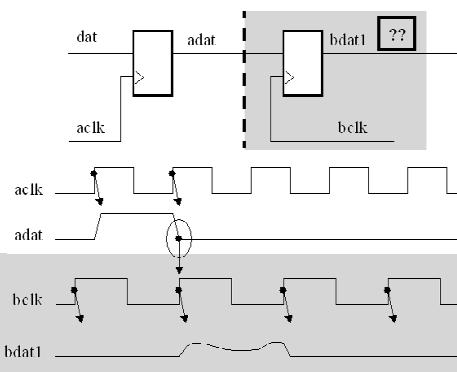
\includegraphics[width=0.55\textwidth]{CDC.png}
  \caption[\textit{Clock Domain Crossing} ]{\textit{Clock Domain Crossing} (fonte: \cite{CDC})}
  \label{fig:airbus1}
\end{figure}

Quando o sinal "adat" proveniente do domínio associado ao relógio "aclk" é capturado pelo registo no domínio associado a "bclk", o sinal à saída do registo pode passar por um período de metaestabilidade no qual flutua instavelmente entre bandas de valores proibidos. Entrando neste estado, não há garantias de que o sinal colapse para o valor lógico correto num período suficientemente reduzido de tempo que permite o normal funcionamento do circuito. O sinal metaestável pode propagar pelo circuito, ser capturado com diferentes valores em registos paralelos e consequentemente gerar uma disrupção no desejado funcionamento do circuito lógico. \par 
Em CDC, é muito improvável que possa ser evitado o aparecimento da metaestabilidade, no entanto, é possível contornar as suas consequências com recurso a técnicas para isso desenvolvidas. A mais básica e conhecida é a inserção de sincronizadores no circuito. Estes consistem numa sequência de registos associados ao domínio de relógio de destino, como se exemplifica na figura 7.2.

\begin{figure}[!htb]
  \centering
  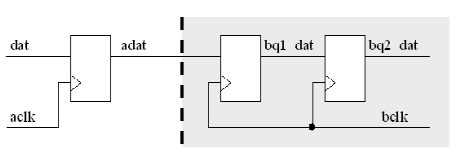
\includegraphics[width=0.65\textwidth]{synch.png}
  \caption[Sincronizador ]{Sincronizador (fonte: \cite{CDC})}
  \label{fig:airbus1}
\end{figure}


Recorrendo a um sincronizador suficientemente longo, é esperado que a metaestabilidade seja resolvida internamente ao mesmo, e que o correto valor do sinal seja, mais ou mais cedo, capturado à entrada do sincronizador. \par
Os sincronizadores servem, como descrito, quando o sinal a transitar entre domínios contém apenas um bit. No entanto, se se pretender transitar sinais com vários bits como, por exemplo, o sinal TXD da interface GMII, estes não são adequados. Ainda que previnam a metaestabilidade, não há garantia de que os vários bits sejam capturados pelo sincronizador num mesmo flanco de relógio. Para fazer a transição de domínios do referido sinal foram implementadas filas assíncronas. Uma ilustração do esquema interno de uma fila assíncrona pode ser observado na figura 7.3

\begin{figure}[h]
  \centering
  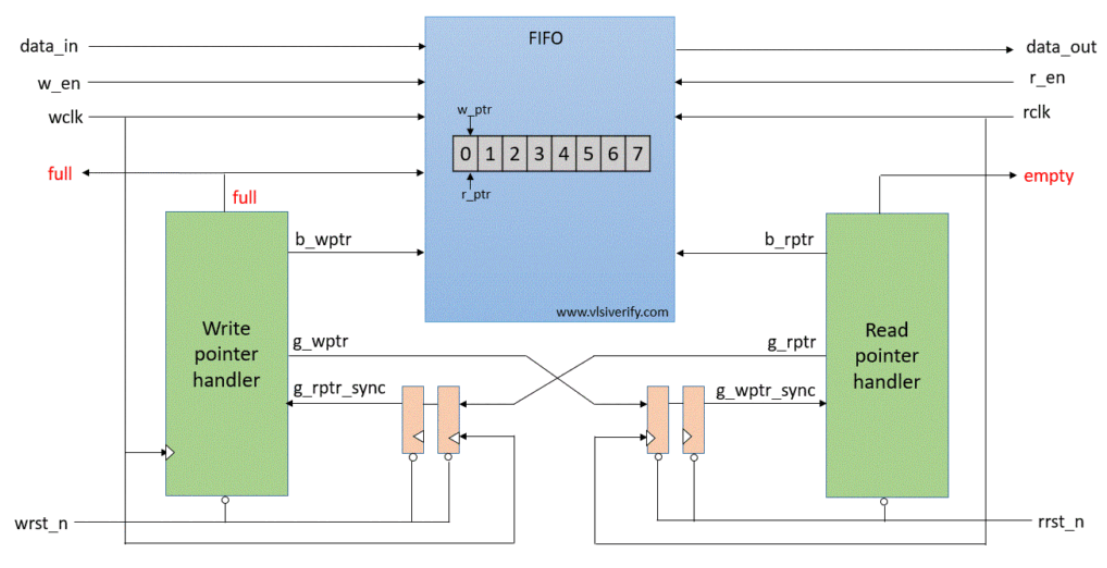
\includegraphics[width=0.9\textwidth]{AsyncFIFO.png}
  \caption[Fila assíncrona]{Fila assíncrona}
  \label{fig:airbus1}
\end{figure}


O esquema interno da fila assíncrona inclui um bloco de memória de profundidade variável, sincronizadores, e dois módulos responsáveis por gerenciar os ponteiros de escrita e leitura. O ponteiro de leitura dá a indicação da posição na fila de onde será efectuada a seguinte leitura, da mesma forma que o ponteiro de escrita dá a indicação da posição na fila da escrita seguinte. Após uma escrita o ponteiro de escrita é incrementado, tal como o ponteiro de leitura após uma leitura. A fila encontra-se cheia ou vazia quando os dois ponteiros indicam a mesma posição na fila. Para distinguir uma situação da outra um bit extra é adicionado ao ponteiro de escrita, duplicando a quantidade de posições que podem por si ser indicadas, de forma a trazer a indicação de que o referido ponteiro deu uma volta extra na fila em relação ao ponteiro de leitura. A comparação entre os dois ponteiros é efectuada pelos módulos denominados \textit{Write Pointer handler} e \textit{Read pointer handler}, que se encontram em domínios de relógio diferentes. Para transitar entre os dois domínios, todos os bits dos ponteiros passam por sincronizadores, como se observa na imagem. Como explicado previamente, tal não é possível se se tentar transitar dados, no entanto, para ponteiros isso é alcançável recorrendo a contadores de Gray. Estes contam segundo um código binário na qual entre dois valores consecutivos apenas há a mudança no valor lógico de um dos bits, ou seja, a distância de Hamming entre dois valores consecutivos é sempre de um. Na tabela 8.1 pode-se observar o código de Gray para os números entre 0 e 15, bem como o bit do código que se altera em cada transição. 

\begin{table}[H]
\begin{center} 
\begin{tabular}{|l|l|l|l|l|}

    \hline
    Decimal &  3 & 2 & 1 & 0 \\
    \hline
    0 & 0 & 0 & 0 & 0 \\
    \hline
    1 & 0 & 0 & 0 & \cellcolor{blue!25}1 \\
    \hline
    2 & 0 & 0 & \cellcolor{blue!25}1 & 1 \\
    \hline
    3 & 0 & 0 & 1 & \cellcolor{blue!25}0 \\
    \hline
    4 & 0 & \cellcolor{blue!25}1 & 1 & 0 \\
    \hline
    5 & 0 & 1 & 1 & \cellcolor{blue!25}1 \\
    \hline
    6 & 0 & 1 & \cellcolor{blue!25}0 & 1 \\
    \hline
    7 & 0 & 1 & 0 & \cellcolor{blue!25}0 \\
    \hline
    8 & \cellcolor{blue!25}1 & 1 & 0 & 0 \\
    \hline
    9 & 1 & 1 & 0 & \cellcolor{blue!25}1 \\
    \hline
    10 & 1 & 1 & \cellcolor{blue!25}1 & 1 \\
    \hline
    11 & 1 & 1 & 1 & \cellcolor{blue!25}0 \\
    \hline
    12 & 1 & \cellcolor{blue!25}0 & 1 & 0 \\
    \hline
    13 & 1 & 0 & 1 & \cellcolor{blue!25}1 \\
    \hline
    14 & 1 & 0 & \cellcolor{blue!25}0 & 1 \\
    \hline
    15 & 1 & 0 & 0 & \cellcolor{blue!25}0 \\
    \hline
    0 & \cellcolor{blue!25}0 & 0 & 0 & 0 \\
    \hline
    
\end{tabular}
\end{center}
\caption{Contador de Gray}\label{Contador de Gray}
\end{table}

\

Como nestes apenas há alteração no valor de um bit aquando do incremento do contador, o valor ponteiro pode demorar uma quantidade variável de ciclos a transitar para o outro domínio, mas nunca transitará com um valor inválido por dois bits diferentes serem capturados em momentos diferentes. As indicações de que a fila está cheia ou vaziam podem demorar uma quantidade indesejável de ciclos a atualizar, atrasar a escrita e leitura de dados na fila, no entanto, nunca se perderão dados. \par 
As filas assíncronas foram posicionadas imediatamente a seguir à recepção dos sinais da interface GMII, permitindo que toda a lógica necessária para receber, armazenar e retransmitir as tramas pudesse operar sobre um único domínio de relógio. A correta instalação das filas e consequente eliminação de possíveis problemas associados a CDC foi verificada com recurso ao \textit{software} \textit{Spyglas} desenvolvido pela \textit{Synopsys}.   



\section{Síntese}

O comutador foi desenvolvido prevendo a implementação futura do mesmo numa FPGA da Intel. Para comprovar a adequação da arquitectura do comutador para FPGA foi feita uma implementação do mesmo na placa de desenvolvimento de FPGA CYCLONE 10GX 10CX220YF780E5G. Esta é uma FPGA de gama média cujos recursos disponibilizados incluem 220000 \textit{lookup-tables} e 11740 kb de memória providenciados por 587 blocos de memória RAM de 20 kb. Sendo a FPGA da Intel, a implementação do comutador na mesma foi efectuada através do \textit{software} Quartus Prime. Na tabela 8.1 é possível observar os recursos necessários para a implementação do comutador na FPGA para diferentes quantidades de portos e em situações de inclusão ou ausência de filas assíncronas. \par   


Na tabela 7.2 podem ser observados recursos necessários para implementação em FPGA para diferentes quantidades de portos e com a possível adição de do suporte para o funcionamento como \textit{Transparent Clock}. Para todas as implementações foram definidos \textit{buffer}s compostos por 30 segmentos de 256 octetos, VOQs com 4 posições e duas prioridades diferentes, tabela de endereços com 128 \textit{buffer}'s circulares de 8 elementos, processador do iSLIP de um único andar, e sem inclusão de contadores e filas assíncronas. A síntese de versões do comutador com uma quantidade mais elevada de portos não foi possível devido à exaustão dos recursos da FPGA.

\begin{table}[h]
\begin{center}
\begin{tabular}{|l|l|}

    \hline
    &    \\
    \hline
     & \\
    \hline
     &   \\
    \hline
     &   \\
    \hline
     &  \\
    \hline
     &  \\
    \hline
    
\end{tabular}
\end{center}
\caption{Recursos da FPGA necessários para a síntese do comutador}\label{Recursos da FPGA necessários para a síntese do comutador}
\end{table}